\documentclass{article}
\usepackage[margin=.5in]{geometry}
\usepackage{amsfonts}
\usepackage{amssymb}
\usepackage{amsmath}
\usepackage{graphicx}
\usepackage{algorithm}
\usepackage{algpseudocode}

\begin{document}
\begin{center}
{\huge \bf CS 6350 Midterm Review}
\end{center}


\hspace{-1.5em}{\large \bf General Supervised Learning}
\begin{itemize}
\item Supervised learning, instance spaces, label spaces, concept and hypothesis spaces
	\begin{itemize}
	\item {\bf Supervised learning:} 
		\begin{itemize}
		\item Given some training examples in the form $\left< x,f(x)\right>$, with $f$ being unknown
		\item Typically, the input $x$ is represented in the {\em feature space}, for example $x\in \{0,1\}^{n}\text{ or }x\in \mathbb{R}^{n}$
		\item For a training example $x$, the value of $f(x)$ is called its {\em label}
		\item \underline{Goal:} Find a good approximation for $f$
		\end{itemize}
	\item {\bf Instance spaces:} The set of the examples and features that are going to be looked at
	\item {\bf Label spaces:} The total set of possible labels that each instance can have
	\item {\bf Concept and Hypothesis spaces:}
		\begin{itemize}
		\item {\bf Hypothesis space:} All of the possible functions that the learning algorithm is going to be searching over
		\item {\bf Concept space:} 
		\end{itemize}
	\end{itemize}
\item Understanding why we need to restrict hypothesis spaces
	\begin{itemize}
	\item Choose a hypothesis space that is smaller than the space of all functions. The functions that are choosen are done by either prior knowledge or by guessing. It also needs to be flexible enough to work with the data and not too small that nothing agrees with it.
	\item For example, in the case of boolean functions, can do only {\em simple conjunctions}, pick {\em m-of-n rules} where you pick a set of $n$ variables, of which at least $m$ need to be true, linear functions, etc.
	\end{itemize}
\item General issues in supervised learning: hypothesis spaces, representation (i.e. features), learning algorithms
	\begin{itemize}
	\item {\bf Hypothesis spaces:} If the hypothesis space is too large, then learning can not be done because there are too many functions to search over. Therefore, to be able to learn, the hypothesis space must be restricted to a smaller subset so that it is possible to learn.
	\item {\bf Representation/features:} Need features that represent the data well. Features that aren't present in a lot of the data {\em or} have too common of a value are not good features.
	\item {\bf Learning algorithms:} The right learning algorithm needs to be choosen such that it can learn from the data well and not be excessive in resource usage. Also you want an algorithm that doesn't overfit the data and has a high success rate.
	\end{itemize}
\end{itemize}


\hspace{-1.5em}{\large \bf Decision Trees}
\begin{itemize}
\item What is a decision tree? What can they represent?
	\begin{itemize}
	\item {\bf Decision tree:} A {\em hierarchical data structure} that represents data using a divide-and-conquor strategy. It can be used as a hypothesis class for non-parametric classification or regression. 

	\underline{General Idea:} Given a collection of examples, learn a decision tree that represents it.
	\item Decision trees are a family of classifiers for instances that are represented by feature vectors (i.e. vectors of attributes)
	\item {\em Nodes} are tests for feature vectors
	\item There is one {\em branch} for every value that the feature can take
	\item {\em Leaves} of the tree specify the class labels
	\end{itemize}
\item How to predict with a decision tree
	\begin{itemize}
	\item At the root node, you're given a test, you then follow the branch for the correct answer for that one node. Decision trees need not be binary!
	\end{itemize}
\item Expressivity, counting the number of decision trees
	\begin{itemize}
	\item {\bf Expressivity:} 
	\end{itemize}
\item Dealing with continuous features
	\begin{itemize}
	\item You would have ranges of values that fall in to each node. For example:
	\begin{center}
	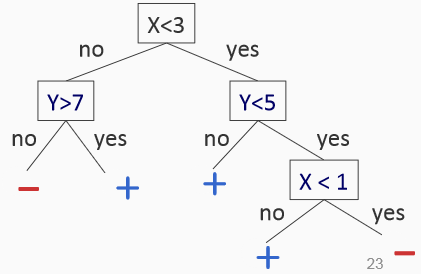
\includegraphics[width=.3\textwidth]{continuous.png}
	\end{center}
	\end{itemize}
\item Learning Algorithm: The ID3 algorithm entropy information gain
	\begin{itemize}
	\item The ID3 Algorithm is based on the {\em entropy} of each attribute

	{\bf ID3}($S$, {\tt Attributes}, {\tt Label}):

		\begin{enumerate}
		\item {\bf If} all examples have the same label:
		
		\hspace{2em}{\bf Return} a single node tree with the label
		\item {\bf Else:}
			\begin{enumerate}
			\item Create a \verb~Root Node~ for the tree
			\item \verb~A~ = attribute in \verb~Attributes~ that {\em \underline{best}} classifies $S$
			\item {\bf for each} possible value $\nu$ that \verb~A~ can take:
				\begin{enumerate}
				\item Add a new tree branch corresponding to \verb~A~ $=\nu$
				\item Let $S\nu$ be the subset of examples in $S$ with \verb~A~ $ =\nu$
				\item {\bf If} $S\nu\in\varnothing$:
				
				\hspace{1em}Add leaf node with the common value of \verb~Label~ in $S$
	
				{\bf Else}:

				\hspace{1em} Below this branch add the subtree \verb~ID3~($S\nu$,{\tt Attributes}$-\{${\tt A}$\}$,{\tt Label})
				\end{enumerate}
			\item {\bf Return} \verb~Root Node~
			\end{enumerate}
		\end{enumerate}
	\item {\bf Entropy and Information Gain:}
		\begin{itemize}
		\item {\em Entropy} is the set of examples $S$ with respect to binary classification is
		\begin{align*}
		Entropy(S) &= H(S) = -p_{+}\log_{2}\left(p_{+}\right)-p_{-}\log_{2}\left(p_{-}\right)\quad \left\{\begin{matrix}
p_{+}\text{ is the porportion of positive examples} \\\ \\
p_{-}\text{ is the proportion of negative examples}
\end{matrix}\right.\\
		Gain(S,A) &= Entropy(S) - \sum_{\nu\in\text{Values}}\frac{\left|S_{\nu}\right|}{\left| S\right|}Entropy\left(S_{\nu}\right)\\
		&S_{\nu}:  \ \ \text{The subset of examples where the value of attribute $A$ is set to value $\nu$}
		\end{align*}
		\end{itemize}
	\item The root attribute that should be choosen is the attribute with the highest information gain
	\end{itemize}
\item Overfitting (applicable not just to decision trees) and how to deal with it when training decision trees
	\begin{itemize}
	\item The learning algorithm fits the noise in the data. Irrelevant attribuytes or noisy examples influence the choice of the hypothesis
	\item May lead to poor performance on future examples
	\item Decision trees are notorous for overfitting, so the solution to this is to favor simpler (shorter) hypotheses as fewer shorter trees are less likely to fit better by coicidence
	\end{itemize}
\item Dealing with missing features
	\begin{itemize}
	\item Using the most common value oif the attribute in the data
	\item Using the most common value of the attribute among all examples with the same output
	\item Using fractional counts of all the attributes
	\item {\em Test time}: Use the same method
	\end{itemize}
\item When to use decision trees
	\begin{itemize}
	\item Binary classifications? Small hypothesis spaces?
	\end{itemize}
\end{itemize}


\hspace{-1.5em}{\large \bf Nearest Neighbors}
\begin{itemize}
\item Instance based learning. How to predict? Importance of representation
	\begin{itemize}
	\item Training examples are vectors $\mathbf{x}_{i}$ associated with a label $y_{i}$
	\item {\em Learning}: Just store all the training examples
	\item {\em Prediction}: For a new example $\mathbf{x}$, find the training example $\mathbf{x}_{i}$ that is {\em closest} to $\mathbf{x}$ and predict the label of $\mathbf{x}$ with the label $y_{i}$ associated with $\mathbf{x}_{i}$.
	\begin{itemize}
		\item {\em Classification}: Every neighbor votes on the label. Predict the most frequent label among the neighbors.
		\item {\em Regression}: Predict the mean value
	\end{itemize}
	\end{itemize}
\item Different definitions of distance
	\begin{itemize}
	\item Euclidean Distance
	\begin{align*}
	\left|\left| \mathbf{x_{1}} - \mathbf{x_{2}}\right|\right|_{2} = \sqrt{\sum_{i=1}^{n}\left(\mathbf{x_{1,i}}-\mathbf{x_{2,i}}\right)^{2}}
	\end{align*}
	\item Manhattan Distance
	\begin{align*}
	\left|\left| \mathbf{x_{1}} - \mathbf{x_{2}}\right|\right|_{1} = \sum_{i=1}^{n}\left|\mathbf{x_{1,i}}-\mathbf{x_{2,i}}\right|
	\end{align*}
	\item $L_{p}$-Norm
	\begin{align*}
	\left|\left| \mathbf{x_{1}} - \mathbf{x_{2}}\right|\right|_{p} = \left( \sum_{i=1}^{n}\left|\mathbf{x_{1,i}}-\mathbf{x_{2,i}} \right|^{p} \right)^{\frac{1}{p}}
	\end{align*}
	\end{itemize}
\item Dealing with symbolic features
	\begin{itemize}
	\item words
	\end{itemize}
\item Choosing $k$ for $k$-NN
	\begin{itemize}
	\item words
	\end{itemize}
\item Practical aspects: Feature normalization could be important
	\begin{itemize}
	\item words
	\end{itemize}
\item Advantages and disadvantages
	\begin{itemize}
	\item words
	\end{itemize}\item Voronoi diagrams
\item Curse of dimensionality (applicable beyond nearest neighbor algorithms)
	\begin{itemize}
	\item words
	\end{itemize}
\end{itemize}

\hspace{-1.5em}{\large \bf Linear Classifiers}
\begin{itemize}
\item What are they? Why are they interesting?
	\begin{itemize}
	\item words
	\end{itemize}
\item What can they express? What can they not express?
	\begin{itemize}
	\item words
	\end{itemize}
\item Geometry
	\begin{itemize}
	\item words
	\end{itemize}
\item Feature expansion to predict a broader set of functions
	\begin{itemize}
	\item words
	\end{itemize}
\end{itemize}

\hspace{-1.5em}{\large \bf Mistake Bound Learning}
\begin{itemize}
\item One way of asking how god is your classifier
	\begin{itemize}
	\item words
	\end{itemize}
\item The general structure of an online learning algorithm
	\begin{itemize}
	\item words
	\end{itemize}
\item Goal: Counting Mistakes. What is a mistake bound algorithm
	\begin{itemize}
	\item words
	\end{itemize}
\item Halving algorithm
	\begin{itemize}
	\item words
	\end{itemize}
\item Perceptron algorithm, geometry of the update, margin, Novikoff's theorem, variants
	\begin{itemize}
	\item words
	\end{itemize}
\item Winnow algorithm, mistake bound, balanced winnow
	\begin{itemize}
	\item words
	\end{itemize}
\item Perceptron vs. Winnow
	\begin{itemize}
	\item words
	\end{itemize}
\end{itemize}

\hspace{-1.5em}{\large \bf Batch Learning}
\begin{itemize}
\item Assumption that train and test examples are drawn from the same distribution 
	\begin{itemize}
	\item words
	\end{itemize}
\item How it is different from mistake bound learning
	\begin{itemize}
	\item words
	\end{itemize}
\end{itemize}
\end{document}
